\section{Tema 2: Cinemática de la partícula fluida}

\subsection{Repaso operador nabla}
En cartesianas nabla se define como:

\[\vec\nabla=\frac{\partial}{\partial x}\vec i + \frac{\partial}{\partial y}\vec j +\frac{\partial}{\partial z}\vec k\]

\begin{itemize}
	\item Aplicado a un campo escalar $\Phi = f(x,y,z)$
	
	\begin{itemize}
		\item Operador gradiente
		\[\vec\nabla \Phi = \left(\frac{\partial}{\partial x}\vec i + \frac{\partial}{\partial y}\vec j +\frac{\partial}{\partial z}\vec k\right) \Phi\]
No es un operador conmutativo.
\item Laplaciano: 
\[\vec\nabla^2=\frac{\partial^2}{\partial x^2}+\frac{\partial^2}{\partial y^2}+\frac{\partial^2}{\partial z^2}\]

\[\vec\nabla^2\Phi=\Delta\Phi=\frac{\partial^2\Phi}{\partial x^2}+\frac{\partial^2\Phi}{\partial y^2}+\frac{\partial^2\Phi}{\partial z^2}\]
	\end{itemize}
	
	\item Aplicado a un campo vectorial $\vec\Phi = \phi_x(x,y,z)\vec i+\phi_y(x,y,z)\vec j+\phi_z(x,y,z)\vec z$
	\begin{itemize}
		\item Divergencia
		\[\vec\nabla \cdot \vec\Phi = \frac{\partial \phi_x}{\partial x} + \frac{\partial \phi_y}{\partial y} + \frac{\partial \phi_z}{\partial z}\]
		
		\item Rotacional
		
		\[
		\vec\nabla \times \vec\Phi = \begin{vmatrix}
			\vec i & \vec j & \vec k \\
			\frac{\partial}{\partial x} & \frac{\partial}{\partial y} & \frac{\partial}{\partial z} \\
			\phi_x & \phi_y & \phi_z \\
		\end{vmatrix}
		\]
		\item Gradiente 
		\setlength{\arraycolsep}{1.5pt}
		\renewcommand{\arraystretch}{1.5}
		\[\vec\nabla  \vec\Phi = \begin{bmatrix}
			\frac{\partial \phi_x}{\partial x} & \frac{\partial \phi_x}{\partial y} & \frac{\partial \phi_x}{\partial z} \\
			\frac{\partial \phi_y}{\partial x} & \frac{\partial \phi_y}{\partial y} & \frac{\partial \phi_y}{\partial z} \\
			\frac{\partial \phi_z}{\partial x} & \frac{\partial \phi_z}{\partial y} & \frac{\partial \phi_z}{\partial z} \\
		\end{bmatrix}\]
		
	\end{itemize}
	\item Relaciones algebraicas
	\begin{enumerate}
		\item $\vec{\nabla}(\varphi \phi) =\varphi\vec{\nabla}\phi+\phi\vec{\nabla}\varphi$
		\item $\vec{\nabla} \times \left(\vec{\nabla} \phi\right)=0$
		\item $\vec{\nabla} \cdot \left(\vec{\nabla} \times \vec{\Phi}\right) =0$
		\item $\left(\vec{\Phi}  \cdot \vec{\nabla}\right)\vec{\Phi}=\vec{\nabla} \frac{\left|\vec\Phi \right|}{2}^2-\vec\Phi \times \left(\vec{\Phi}  \cdot \vec{\nabla}\right) $ 
	\end{enumerate}
\end{itemize}

\subsection{Conceptos fundamentales}
\begin{figure}[H]
	\centering
	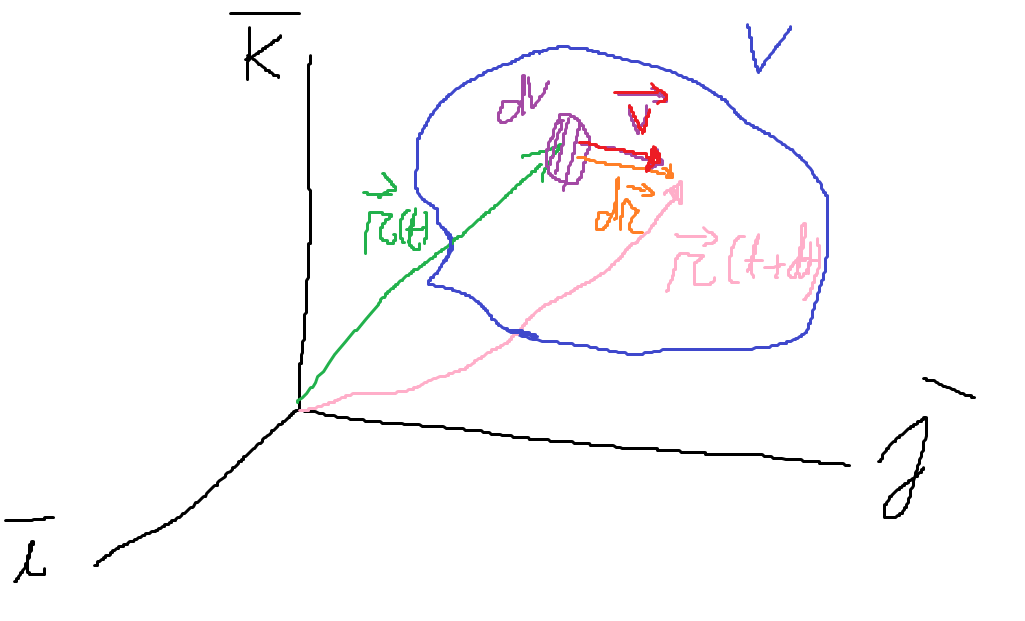
\includegraphics[width=0.5\linewidth]{imagenesTema2/magnitudesFundamentales}
	\caption{Magnitudes fundamentales.}
	\label{fig:magnitudesfundamentales}
\end{figure}

\begin{enumerate}
	\item \underline{\textbf{Trayectoria}}: Se determina el vector posición a partir de la velocidad. Esta ligada al enfoque lagrangiano. Tiene realidad física.
	\[\vec{v}=\frac{d\vec{r}}{dt} \rightarrow \vec{r}(t=0)=\vec{r_0}\]
	
	\item \underline{\textbf{Senda}}: Camino que se recorre. Es independiente del tiempo y se obtiene eliminando el tiempo t de la trayectoria. Tiene realidad física.
	
	\item \underline{\textbf{Línea de corriente}}: No tiene realidad física. Se basa den el enfoque euleriano.
	\[d\vec{r}//\vec{v}\]
	\[\vec{r}=x\vec{i}+y\vec{j}+z\vec k \rightarrow d\vec{r}=dx\vec{i}+dy\vec{j}+dz\vec{k}\]
	\[\vec{v}=v_x\vec{i}+v_y\vec{j}+v_z\vec{k}\]
	\[Si \ d\vec{r} // \vec{v} \rightarrow \vec{v} \times d\vec{r}=0= \begin{vmatrix}
		\vec i & \vec j & \vec k \\
		v_x & v_y & v_z \\
		dx & dy & dz \\
	\end{vmatrix}= \left(v_ydz-v_zdy\right)\vec{i} +\left(v_zdx-v_xdz\right)\vec{j}+\left(v_xdy-v_ydx\right) \]
	
	\[\therefore\frac{dz}{v_z}=\frac{dy}{v_y} \rightleftharpoons \frac{dz}{v_z}=\frac{dx}{v_x} \rightleftharpoons \frac{dx}{v_x}=\frac{dy}{v_y} \]
\end{enumerate}

\subsection{Clasificación flujos}
\begin{enumerate}
	\item \underline{\textbf{Enfoque elección de coordenadas}}
	\begin{enumerate}
		\item Lagrangiano: Enfoque de seguir a la partícula. 
		\[\vec{v}=\vec{v}(t(\vec{r}))=\vec{v}(t)\]
		\item Euclídeo: Enfoque de centrarse en el espacio.
		\[\vec{v}=\vec{v}(\vec{r},t)=v_x(x,y,z,t)\vec{i}+v_y(x,y,z,t)\vec{j}+v_z(x,y,z,t)\vec{k}\]
	\end{enumerate}
	\item \underline{\textbf{Dirección}}
	\begin{enumerate}
		\item 3 direcciones ($\vec{i},\vec{j},\vec{k}$): 
		\begin{itemize}
			\item Campo vectorial tridireccional.
		\end{itemize}
		\item 2 direcciones ($\vec{i},\vec{k}$):
		\begin{itemize}
			\item Campo vectorial bidireccional.
		\end{itemize}
		\item 1 dirección ($\vec{j}$):
		\begin{itemize}
			\item Campo vectorial unidireccional.
		\end{itemize}
	\end{enumerate}
	\item \underline{\textbf{Espacio}}
	\begin{enumerate}
		\item Si alguna componente depende de x, y, z: 
		\begin{itemize}
			\item Campo vectorial tridimensional.
		\end{itemize}
		\item Si ninguna componente depende de x, y o z: 
		\begin{itemize}
			\item Campo vectorial bidimensional.
		\end{itemize}
		\item Si todas las componentes dependen de x, y o z: 
		\begin{itemize}
			\item Campo vectorial unidimensional o monodimensional.
		\end{itemize}
		\item Si ninguna componente depende de x, y, z: 
		\begin{itemize}
			\item Campo vectorial uniforme o homogéneo.
		\end{itemize}
	\end{enumerate}
	\item \underline{\textbf{Tiempo}}
	\begin{enumerate}
		\item Si alguna componente depende del tiempo:
		\begin{itemize}
			\item Campo vectorial no estacionario o transitorio.
		\end{itemize}
		\item Si ninguna componente depende del tiempo:
		\begin{itemize}
			\item Campo vectorial estacionario.
		\end{itemize}
	\end{enumerate}
\end{enumerate}
\subsection{Derivada sustancial, local y convectiva}
Al operador diferencial de variación temporal se le denomina derivada sustancial, total o material:
\[\frac{D}{Dt}=\frac{\partial}{\partial t}+\left(\vec{v} \cdot \vec{\nabla}\right)\]

\begin{figure}[H]
	\centering
	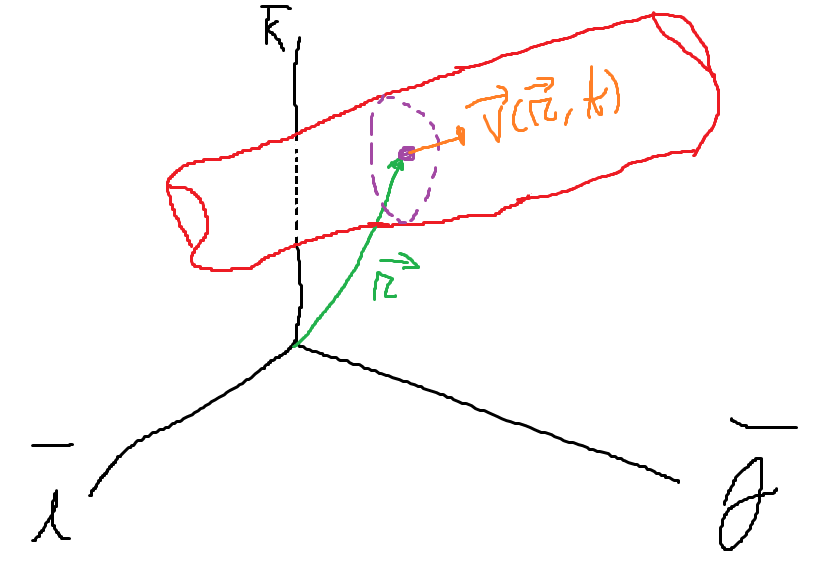
\includegraphics[width=0.5\linewidth]{imagenesTema2/derivadaSustancial}
	\caption{Derivada sustancial.}
	\label{fig:derivadasustancial}
\end{figure}

Sea $\phi=f(\vec{r},t)$ y $\vec{r}=x\vec{i}+y\vec{j}+z\vec{k}$
\[d\phi=\phi(\vec{r}+d\vec{r},t+dt)-\phi(\vec{r},t)=dx\frac{\partial \phi}{\partial x}+dy\frac{\partial \phi}{\partial y}+dz\frac{\partial \phi}{\partial z}+\frac{\partial \phi}{\partial t}dt=d\vec{r} \cdot\vec{\nabla}\phi+\frac{\partial \phi}{\partial t}dt\]

\[\frac{d\phi}{dt}=\vec{v} \cdot\vec{\nabla}\phi +\frac{\partial \phi}{\partial t} \]
\begin{itemize}
	\item Derivada convectiva: $\vec{v} \cdot\vec{\nabla}\phi$
	\item Derivada local o temporal: $\frac{\partial \phi}{\partial t}$
	\item Si $\phi = \vec{v}$
	\[\frac{d\vec{v}}{dt}=(\vec{v} \cdot\vec{\nabla})\vec{v}+\frac{\partial \vec v}{\partial t} \]
	\begin{itemize}
		\item Aceleración convectiva: $(\vec{v} \cdot\vec{\nabla})\vec{v}$
		\[(\vec{v} \cdot\vec{\nabla})\vec{v}=\vec{\nabla}\frac{|\vec{v}|}{2}^2-\vec{v} \times \left(\vec{\nabla}\times\vec{v}\right)\]
		\begin{itemize}
			\item Aceleración modular o debida a cambios del módulo de la velocidad: $\vec{\nabla}\frac{|\vec{v}|}{2}^2$
			\item Aceleración direccional: $-\vec{v} \times \left(\vec{\nabla}\times\vec{v}\right)$
			\begin{itemize}
				\item Vorticidad: $\vec{\omega}= \left(\vec{\nabla}\times\vec{v}\right)$
			
				\item Si la vorticidad es nula, el fluido es irrotacional y existe una función de corriente tal que:
				\[\vec{v}=-\vec{\nabla}\phi \rightarrow \vec{\nabla}\times\left(-\vec{\nabla}\phi\right)=0\]
				\item  En la literatura, a veces en lugar de hablar de vorticidad, se define velocidad de rotación como:
				\[\vec{\Omega}=\frac{\vec{\omega}}{2}\]
			\end{itemize}
		\end{itemize}
		\item Aceleración local: $\frac{\partial \vec v}{\partial t}$
	\end{itemize}
\end{itemize}
\newpage
\subsection{Movimiento diferencial en torno a un punto}
A partir de la figura siguiente, se puede deducir que el movimiento diferencial es:
\[\lim_{{dt \to 0}} d\vec{v}dt=\vec{v}(\vec{r}+d\vec{r},t)dt-\vec{v}(\vec r ,t)dt\]
\begin{figure}[H]
	\centering
	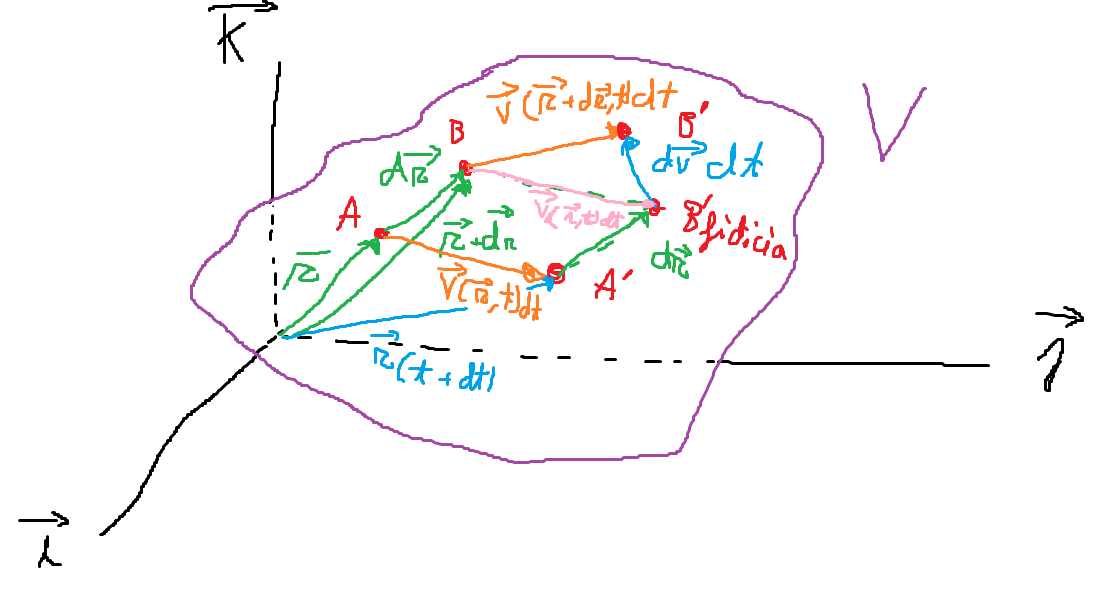
\includegraphics[width=0.7\linewidth]{imagenesTema2/movimientoDiferencial}
	\caption{Magnitudes fundamentales del movimiento diferencial.}
	\label{fig:movimientodiferencial}
\end{figure}
Operando y despreciando el diferencial de tiempo:
\[d\vec{v}=\vec{v}(\vec{r}+d\vec{r},t)-\vec{v}(\vec r ,t)=d\vec{r}\cdot(\vec{\nabla}\vec{v})\]
Donde $\vec{\nabla}\vec{v}$ es el tensor gradiente de la velocidad:
\setlength{\arraycolsep}{1.5pt}
\renewcommand{\arraystretch}{1.5}
\[\vec{\nabla}\vec{v}=\begin{bmatrix}
	\frac{\partial v_x}{\partial x} & \frac{\partial v_x}{\partial y} & \frac{\partial v_x}{\partial z} \\
	\frac{\partial v_y}{\partial x} & \frac{\partial v_y}{\partial y} & \frac{\partial v_y}{\partial z} \\
	\frac{\partial v_z}{\partial x} & \frac{\partial v_z}{\partial y} & \frac{\partial v_z}{\partial z} \\
\end{bmatrix}=\frac{1}{2}\left[\vec{\nabla}\vec{v}+\left(\vec{\nabla}\vec{v}\right)^t\right]+\frac{1}{2}\left[\vec{\nabla}\vec{v}-\left(\vec{\nabla}\vec{v}\right)^t\right]=\overline{\overline{\xi}}+\overline{\overline{\gamma}}\]
Las variables que aparecen, son $\overline{\overline{\xi}}$ el tensor de velocidad de deformación (simétrico) y $\overline{\overline{\gamma}}$ el tensor de velocidad de rotación.
\setlength{\arraycolsep}{1.5pt}
\renewcommand{\arraystretch}{1.5}
\[\overline{\overline{\xi}}=\begin{bmatrix}
	\frac{\partial v_x}{\partial x} & \frac{1}{2}\left(\frac{\partial v_x}{\partial y}+\frac{\partial v_y}{\partial x}\right) & \frac{1}{2}\left(\frac{\partial v_x}{\partial z}+\frac{\partial v_z}{\partial x}\right) \\
	\frac{1}{2}\left(\frac{\partial v_x}{\partial y}+\frac{\partial v_y}{\partial x}\right) & \frac{\partial v_y}{\partial y} & \frac{1}{2}\left(\frac{\partial v_y}{\partial z} +\frac{\partial v_z}{\partial y}\right) \\
	\frac{1}{2}\left(\frac{\partial v_x}{\partial z}+\frac{\partial v_z}{\partial x}\right) & \frac{1}{2}\left(\frac{\partial v_y}{\partial z} +\frac{\partial v_z}{\partial y}\right) & \frac{\partial v_z}{\partial z} \\
\end{bmatrix}\]
\setlength{\arraycolsep}{1.5pt}
\renewcommand{\arraystretch}{1.5}
\[\overline{\overline{\gamma}}=\begin{bmatrix}
0 & \frac{1}{2}\left(\frac{\partial v_x}{\partial y}-\frac{\partial v_y}{\partial x}\right) & \frac{1}{2}\left(\frac{\partial v_x}{\partial z}-\frac{\partial v_z}{\partial x}\right) \\

	-\frac{1}{2}\left(\frac{\partial v_x}{\partial y}-\frac{\partial v_y}{\partial x}\right) & 0 & \frac{1}{2}\left(\frac{\partial v_y}{\partial z} -\frac{\partial v_z}{\partial y}\right) \\
	
	-\frac{1}{2}\left(\frac{\partial v_x}{\partial z}-\frac{\partial v_z}{\partial x}\right) & -\frac{1}{2}\left(\frac{\partial v_y}{\partial z} -\frac{\partial v_z}{\partial y}\right) & 0 \\
\end{bmatrix}\]
Por tanto, aplicado al movimiento:
\[d\vec{v}=d\vec{r}\cdot(\vec{\nabla}\vec{v})=d\vec{r}\cdot\overline{\overline{\xi}}+d\vec{r}\cdot\overline{\overline{\gamma}}\]
Donde:
\begin{itemize}
	\item Movimiento velocidad de deformación: $d\vec{r}\cdot\overline{\overline{\xi}}$ que representa las deformaciones lineales (diagonal) y angulares (fuera de la diagonal).
	\begin{itemize}
		\item Si la traza de $\overline{\overline{\xi}}$ es nula, el fluido es incompresible y, por tanto de densidad constante.
	\end{itemize}
	\item Movimiento velocidad de rotación: $\overline{\overline{\gamma}}$ que representa el movimiento del fluido como si fuera un sólido rígido.
	\begin{itemize}
		\item Se puede relacionar este tensor con la vorticidad y se demuestra que:
		\[\overline{\overline{\gamma}} =\frac{1}{2}\vec{\omega}\times d \vec{r}=\left(\vec{\nabla}\times\vec{v}\right)\times d \vec{r}=\begin{bmatrix}
			0 & -\frac{1}{2}\omega_z & \frac{1}{2}\omega_y \\
			\frac{1}{2}\omega_z & 0 & -\frac{1}{2}\omega_x\\	
			-\frac{1}{2}\omega_y & \frac{1}{2}\omega_x & 0 \\
		\end{bmatrix}\]
	\end{itemize}
\end{itemize}
\subsection{Movimiento de la partícula fluida en una dirección}
Se parte de la expresión deducida anteriormente pero expresando el $d\vec{r}$ mediante módulo dirección, esta expresión, también se suele denominar movimiento vectorial:
\[d\vec{v}=d\vec{r}\cdot\left(\vec{\nabla}\vec{v}\right)=d\vec{r}\cdot\left(\overline{\overline{\xi}}+\overline{\overline{\gamma}}\right)=|d\vec{r}|\vec{n}\cdot\left(\overline{\overline{\xi}}+\overline{\overline{\gamma}}\right)\]
\begin{figure}[H]
	\centering
	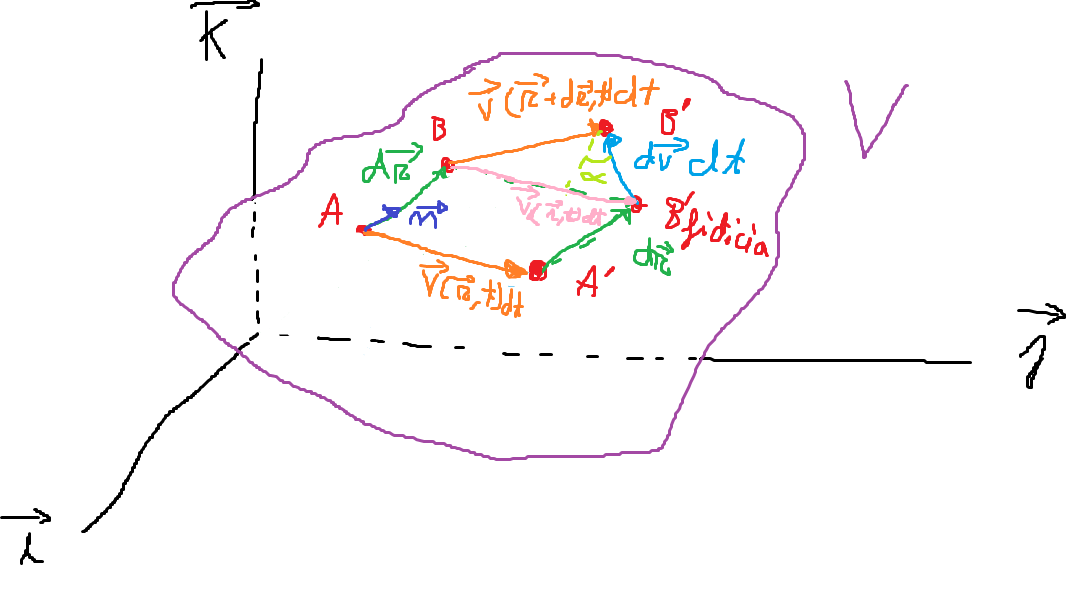
\includegraphics[width=0.7\linewidth]{imagenesTema2/movimientoDireccion}
	\caption{Magnitudes fundamentales del movimiento de la partícula fluida.}
	\label{fig:movimientodireccion}
\end{figure}
Si se aplica a una dirección concreta, también suele denominarse como movimiento escalar:
\[d\vec{v}\cdot\vec{n}=d\vec{r}\cdot\left(\vec{\nabla}\vec{v}\right)=d\vec{r}\cdot\left(\overline{\overline{\xi}}+\overline{\overline{\gamma}}\right)=|d\vec{r}|\vec{n}\cdot\left(\overline{\overline{\xi}}+\overline{\overline{\gamma}}\right)\cdot\vec{n}=\vec{n}\cdot\left(\overline{\overline{\xi}}+\overline{\overline{\gamma}}\right)\cdot\vec{n}\]
Como la dirección no es más que una composición de las distintas direcciones, se puede dividir por coordenadas:
\begin{itemize}
	\item Los términos de deformación:
	\begin{itemize}
		\item Si $\vec{n}=\vec{i}\rightarrow\vec{i}\cdot\overline{\overline{\xi}}\cdot\vec{i}=\xi_{11}$
		\item Si $\vec{n}=\vec{j}\rightarrow\vec{j}\cdot\overline{\overline{\xi}}\cdot\vec{j}=\xi_{22}$
		\item Si $\vec{n}=\vec{k}\rightarrow\vec{k}\cdot\overline{\overline{\xi}}\cdot\vec{k}=\xi_{33}$
	\end{itemize}
	\item Los términos de velocidad de rotación:
	\begin{itemize}
		\item Para todo vector $\vec{n}\cdot\overline{\overline{\gamma}}\cdot\vec{n}=0$
	\end{itemize}
\end{itemize}

